\chapter{Web Technologies}

\label{chap:WebTechnologies}

\section{HyperText Markup Language (HTML)}

HTML is a document markup language for documents that are meant to be displayed in web browsers. The original proposal and implementation in 1989 came from Tim Berners-Lee who was a contractor at CERN at the time \parencite{TBLProposal}. Over the years, the standard has been developed by a range of different entities like the CERN and the Internet Engineering Task Force (IETF). Today, HTML exists as a continuously evolving living standard without specific version releases that is maintained by the Web Hypertext Application Technology Working Group (WHATWG) and the World Wide Web Consortium (W3C) \parencite{HtmlSpec}.

The primary purpose of HTML is to define the content and structure of web pages. This is achieved with the help of HTML elements, which are composed in a hierarchical tree structure and define modular pieces of content that can be interpreted by web browsers. An example of a basic HTML page can be seen in Figure \ref{fig:HTMLStructure}.

\begin{figure}[tp]
    \centering
    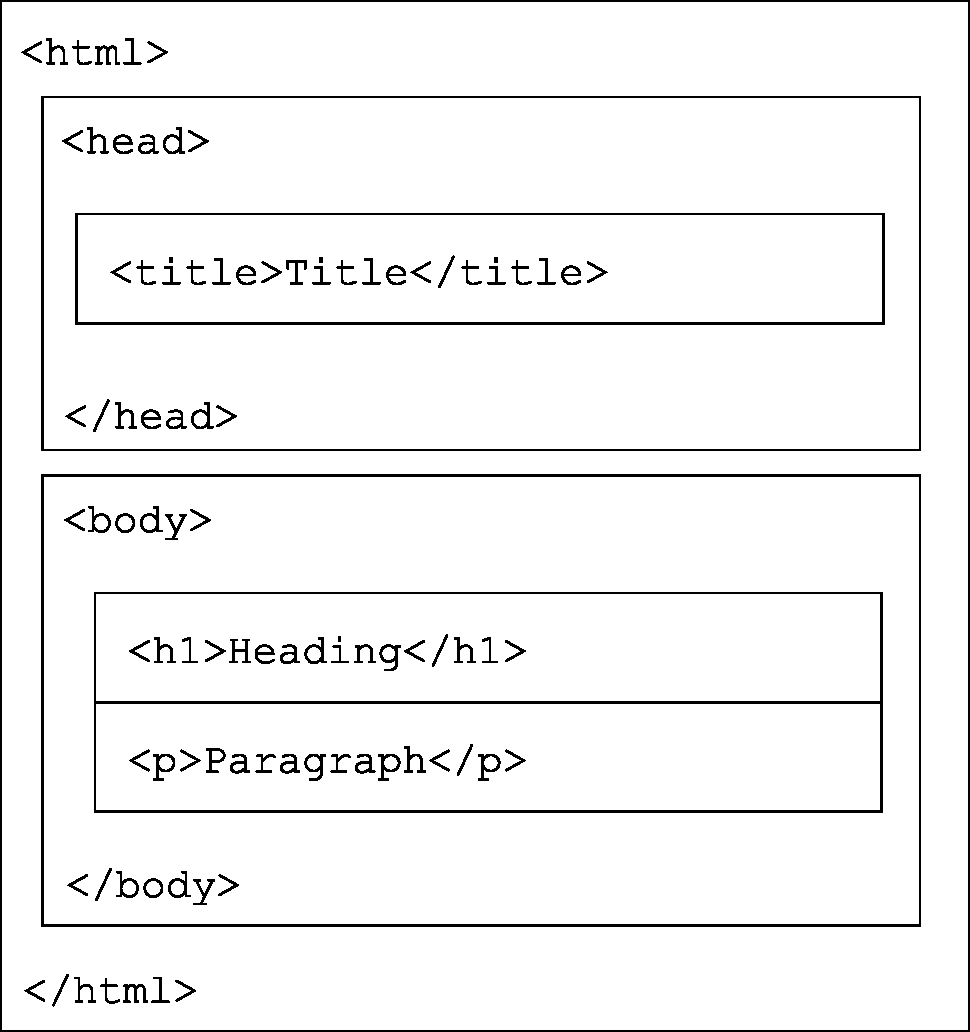
\includegraphics[keepaspectratio,width=\linewidth,height=\halfh]
    {diagrams/html-structure.pdf}

    \caption[Structure of HTML pages]{
        HTML pages are structured as a hierarchical tree of elements which enables the composition of complex structures.
        \imgcredit{Image drawn by the author of this thesis.}
    }
    \label{fig:HTMLStructure}
\end{figure}

A strong pillar of HTML's design is extensibility. There are multiple mechanisms in place to ensure applicability to a vast range of use cases. These mechanisms include:

\begin{itemize}
    \item Specifying classes of elements using the \lstinline{class} attribute. This effectively creates custom elements while still basing them on the most related, already existing elements.
    \item Using \lstinline{data-*} attributes to decorate elements with additional data that can be used by scripts. The HTML standard guarantees that these attributes are ignored by browsers.
    \item Embedding custom data using \lstinline{<script type="">} elements that can be accessed by scripts.
\end{itemize}


\section{Cascading Style Sheets (CSS)}

Cascading Style Sheets (CSS) is a style sheet language that is used to specify the presentation of a HTML document. It can either be embedded directly in HTML documents or it can be defined externally and linked into them. This characteristic of being able to externally describe the presentation of documents yields a lot of flexibility because multiple documents with different content can reuse the same presentation by linking to the same CSS file. 


It can not only be  used to describe the style of elements but also their layout. 

By not directly including presentation features in the HTML standard, a separation of concerns is achieved that improves accessibility and flexibility.

\subsection{Box Layout}
\subsection{Flexbox Layout}
\subsection{Grid Layout}

\section{JavaScript (JS)}

\section{TypeScript (TS)}

\section{Web Graphics}

\subsection{Raster Images}

\TODO{Describe raster images}

\TODO{Mention JPEG}

\TODO{Mention PNG}

\subsection{Scalable Vector Graphics (SVG)}

\TODO{Define detail in which to write about SVG}

\TODO{Describe SVG}

\TODO{Describe filters}

\TODO{Talk about issues with using CSS for styling}



SVG elements can be styled with CSS which is highly convenient as it brings all the benefits of CSS like allowing users to override parts of the styling in their own style sheets. SVG styles defined as CSS can also be animated using CSS animations and transitions. This is recommendable to manual animations using JavaScript because external configuration is inherently supported and the declarative syntax of CSS animations is powerful enough to define complex animations.

% However, SVG 1.1 \TODO{Cite spec} only supports configuration of presentation attributes via CSS and it is not possible to . Other types of attributes, like geometric attributes, can't be styled using CSS and require actual configuaration via HTML attributes. SVG 2 will support styling and animating non-presentation attributes with CSS. \TODO{Add (partial?) list of presentation attributes}\TODO{Add (partial?) list of presentation attributes}

% https://css-tricks.com/svg-properties-and-css/#svg-2
% https://stackoverflow.com/a/14258103


\subsection{Canvas}

\subsection{WebGL}

\section{Layout Engines}

\subsection{Yoga Layout}
\subsection{FaberJS}

\section{Visualization Libraries}

\subsection{Chartist}
\subsection{Highcharts}
\subsection{ECharts}
\subsection{...?}
\subsection{D3}
\TODO{Mention that D3 is successor of Protovis}

\section{Tools}
\subsection{Node}
\subsection{Rollup}
\subsection{Gulp}

